%
% Portuguese-BR vertion
% 
\documentclass{report}

\usepackage{ipprocess}
% Use longtable if you want big tables to split over multiple pages.
\usepackage{longtable}
\usepackage[utf8]{inputenc} 
\usepackage[brazil]{babel} % Uncomment for portuguese
\usepackage{pdflscape} % set ladscape/portrait pdf pages
\usepackage{tikz}
\usepackage{tikz-uml}

\sloppy

\graphicspath{{./pictures/}} % Pictures dir
\makeindex
\begin{document}


%%%%%%%%%%%%%%%%%%%%%%%%%%%%%%%%%%%%%%%%%%%%%%%%%%
%% Building front cover
%%%%%%%%%%%%%%%%%%%%%%%%%%%%%%%%%%%%%%%%%%%%%%%%%%
\DocumentTitle{Documento de Arquitetura}
\Project{Unidade de Operações Aritméticas}
\Organization{Universidade Estadual de Feira de Santana}
\Version{Compilação 1.0}
% Make front cover
\capa
%

%%%%%%%%%%%%%%%%%%%%%%%%%%%%%%%%%%%%%%%%%%%%%%%%%%
%% Revision History
%%%%%%%%%%%%%%%%%%%%%%%%%%%%%%%%%%%%%%%%%%%%%%%%%%
\chapter*{Histórico de Revisões}
  \vspace*{1cm}
  \begin{table}[ht]
    \centering
    \begin{tabular}[pos]{|m{2cm} | m{8cm} | m{4cm}|} 
      \hline
      \cellcolor[gray]{0.9}
      \textbf{Date} & \cellcolor[gray]{0.9}\textbf{Descrição} & \cellcolor[gray]{0.9}\textbf{Autor(s)}\\
      \hline
      25/06/2014 &  Concepção do documento & joaocarlos \\ \hline
    \end{tabular}
  \end{table}

% TOC instantiation
\tableofcontents

%%%%%%%%%%%%%%%%%%%%%%%%%%%%%%%%%%%%%%%%%%%%%%%%%%
%% Document main content
%%%%%%%%%%%%%%%%%%%%%%%%%%%%%%%%%%%%%%%%%%%%%%%%%%
\chapter{Introdução}
  
  \section{Propósito do Documento}
  Este documento descreve a arquitetura do projeto \ipPROCESSProject, incluindo especificações do circuitos internos e máquinas de estados de cada componente. Ele também apresenta diagramas de classe, definições de entrada e saída e diagramas de temporização.O principal objetivo deste documento é definir as especificações do projeto \ipPROCESSProject e prover uma visão geral completa do mesmo.

  \noindent \textcolor{red}{\textit{Informações adicionais podem ser incluídas nesta seção. Entretanto, via de regra, ela não deve se extender por muitos parágrafos.}}

  \section{Stakeholders}
    \textcolor{red}{\textit{Preencher com as informações e papeis da equipe de desenvolvimento.}}
    \FloatBarrier
    \begin{table}[H] 
      \begin{center}
        \begin{tabular}[pos]{|m{6cm} | m{8cm}|} 
          \hline 
          \cellcolor[gray]{0.9}\textbf{Nome} & \cellcolor[gray]{0.9}\textbf{Papel/Responsabilidades} \\ \hline
           &  \\ \hline
        \end{tabular}
      \end{center}
    \end{table} 

\section{Visão Geral do Documento}

O presente documento é apresentado como segue:

  \begin{itemize}
   \item \textbf{Capítulo 2 --} Este capítulo apresenta uma visão geral da arquitetura, com foco em entrada e saída do sistema e arquitetura geral do mesmo;
   \item \textbf{Capítulo 3 --} Este capítulo descreve a arquitetura interna do IP a partir do detalhamento dos seus componentes, definição de portas de entrada e saída e especificação de caminho de dados.
  \end{itemize}


  % inicio das definições do documento
  \section{Definições}
    \FloatBarrier
    \begin{table}[H]
      \begin{center}
        \begin{tabular}[pos]{|m{5cm} | m{9cm}|} 
          \hline
          \cellcolor[gray]{0.9}\textbf{Termo} & \cellcolor[gray]{0.9}\textbf{Descrição} \\ \hline
          RS232                & Protocolo de comunicação serial utilizado em aplicações que requerem transmissão de dados entre elementos conectados à um mesmo canal.                    \\ \hline
        \end{tabular}
      \end{center}
    \end{table}  
  % fim

  % inicio da tabela de acronimos e abreviacoes do documento
  \section{Acrônimos e Abreviações}
    \FloatBarrier
    \begin{table}[H]
      \begin{center}
        \begin{tabular}[pos]{|m{2cm} | m{12cm}|} 
          \hline
          \cellcolor[gray]{0.9}\textbf{Sigla} & \cellcolor[gray]{0.9}\textbf{Descrição} \\ \hline
          TBD      &  To be defined (A ser definido)  \\ \hline
        \end{tabular}
      \end{center}
    \end{table}  
  % fim

\chapter{Visão Geral da Arquitetura}

  \section{Descrição dos Componentes}
  A unidade de processamento a ser desenvolvida é composta a partir dos seguintes componentes:

  \begin{itemize}
    \item \textbf{Serial Controller --} Controlador para comunicação com módulo de transmissão serial através do protocolo RS232.
    \item \textbf{Interface Control --} Interface de controle, responsável por fazer a leitura correta das informações da serial e transmiti-las para a unidade de processamento.
    \item \textbf{Processing Unit --} Unidade responsável pela realização das operações e armazenamento do resultado.
  \end{itemize}

  \section{Diagrama de Classe (Interface)}
  \begin{figure}[H]
    \centering
        \begin{tikzpicture} 
      \umlclass[type=interface]{IP\_Interface}
      { % atributos
        + clock : input bit \\
        + reset : input bit \\
        + rx : input bit \\
        % + tx : output bit \\
        + result\_data : output bit[8] \\
        + overflow : output bit
      }{}
    \end{tikzpicture}
  \end{figure}

  \section{Definições de Entrada e Saída}
  \FloatBarrier
    \begin{center}
      \begin{longtable}[pos]{| l | c | c | m{7cm} |} \hline         
        \multicolumn{1}{|c|}{\cellcolor[gray]{0.9}\textbf{Nome}} & 
        \multicolumn{1}{c|}{\cellcolor[gray]{0.9}\textbf{Tamanho}} & 
        \multicolumn{1}{c|}{\cellcolor[gray]{0.9}\textbf{Direção}} &
        \multicolumn{1}{c|}{\cellcolor[gray]{0.9}\textbf{Descrição}} \\ \hline
        \endfirsthead
        \hline
        \multicolumn{4}{|l|}%
        {{\bfseries continuação da página anterior}} \\
        \hline
        \multicolumn{1}{|c|}{\cellcolor[gray]{0.9}\textbf{Nome}} & 
        \multicolumn{1}{c|}{\cellcolor[gray]{0.9}\textbf{Tamanho}} & 
        \multicolumn{1}{c|}{\cellcolor[gray]{0.9}\textbf{Direção}} &
        \multicolumn{1}{c|}{\cellcolor[gray]{0.9}\textbf{Descrição}} \\ \hline
        \endhead

        \multicolumn{4}{|r|}{{continua na próxima página}} \\ \hline
        \endfoot

        \hline
        \endlastfoot

        clock\_in                & 1   & entrada   & Clock principal do sistema.    \\ \hline
        reset\_in                & 1   & entrada   & Sinal de reset geral do sistema.    \\ \hline
        rx\_in                   & 1   & entrada   & Dado serial da RS232. \\ \hline
        % tx\_out                  & 1   & saída     & Dado serial RS232 a ser transmitido. \\ \hline
        result\_data\_out        & 8   & saída     & Representação do resultado da operação. \\ \hline
        overflow\_out            & 1   & saída     & Sinal indicador de overflow aritmético. \\
      \end{longtable}
    \end{center} 
  \section{Datapath Interno}
    \begin{figure}[H]
      \centering
      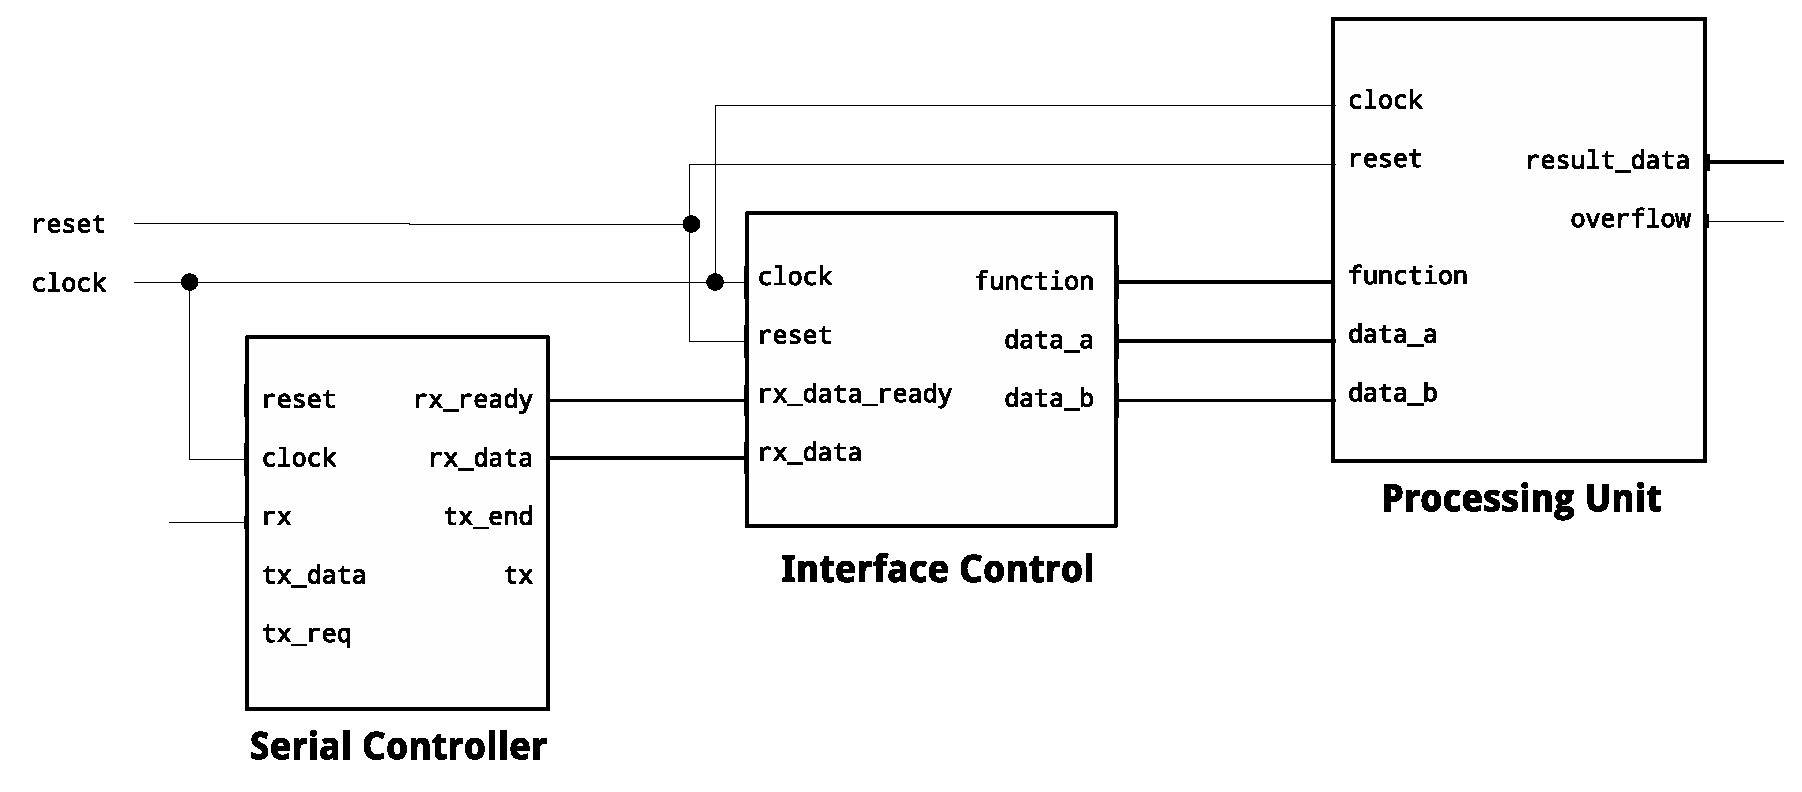
\includegraphics[width=\linewidth]{datapath/ip_datapath.eps}
    \end{figure}

% inicio das descrições de arquitetura para cada componente do sistema
\chapter{Descrição da Arquitetura}

  \section{Unidade de Processamento}

    \subsection{Diagrama de Classe}
      \begin{figure}[H]
      \centering
            \begin{tikzpicture} 
        \umlclass[type=control]{Processing\_Unit}
        { % atributos
          + clock : input bit \\
          + reset : input bit \\
          + data\_a : input bit[8] \\
          + data\_b : input bit[8] \\
          + operation : input bit[TBD] \\          
          + result\_data : output bit[8] \\
          + overflow : output bit \\
          - enable\_result\_reg : reg bit \\
          - reult\_reg : reg bit[8]
        }{ % procedures
          - \underline{<<comb>> process\_operation()} \\
          - <<comb>> setup\_flag() \\
          - <<sequ>> result\_reg\_handler()
        }
      \end{tikzpicture}
    \end{figure}

    \subsection{Definições de Entrada e Saída}
      \FloatBarrier
      \begin{center}
        \begin{longtable}[pos]{| l | c | c | m{7cm} |} \hline         
          \multicolumn{1}{|c|}{\cellcolor[gray]{0.9}\textbf{Nome}} & 
          \multicolumn{1}{c|}{\cellcolor[gray]{0.9}\textbf{Tamanho}} & 
          \multicolumn{1}{c|}{\cellcolor[gray]{0.9}\textbf{Direção}} &
          \multicolumn{1}{c|}{\cellcolor[gray]{0.9}\textbf{Descrição}} \\ \hline
          \endfirsthead
          \hline
          \multicolumn{4}{|l|}%
          {{\bfseries continuação da página anterior}} \\
          \hline
          \multicolumn{1}{|c|}{\cellcolor[gray]{0.9}\textbf{Nome}} & 
          \multicolumn{1}{c|}{\cellcolor[gray]{0.9}\textbf{Tamanho}} & 
          \multicolumn{1}{c|}{\cellcolor[gray]{0.9}\textbf{Direção}} &
          \multicolumn{1}{c|}{\cellcolor[gray]{0.9}\textbf{Descrição}} \\ \hline
          \endhead

          \multicolumn{4}{|r|}{{continua na próxima página}} \\ \hline
          \endfoot

          \hline
          \endlastfoot

          clock\_in                & 1   & entrada   & Clock principal do sistema.    \\ \hline
          reset\_in                & 1   & entrada   & Sinal de reset geral do sistema.    \\ \hline
          data\_a\_in              & 8   & entrada   & Dado do primeiro operando.    \\ \hline
          data\_b\_in              & 8   & entrada   & Dado do segundo operando.    \\ \hline
          operation\_in            & TBD   & entrada   & Código da operação.    \\ \hline
          result\_data\_out        & 8   & saída     & Representação do resultado da operação. \\ \hline
          overflow\_out            & 1   & saída     & Sinal indicador de overflow aritmético. \\
        \end{longtable}
      \end{center} 

    \subsection{Datapath Interno}
      \begin{figure}[H]
        \centering
        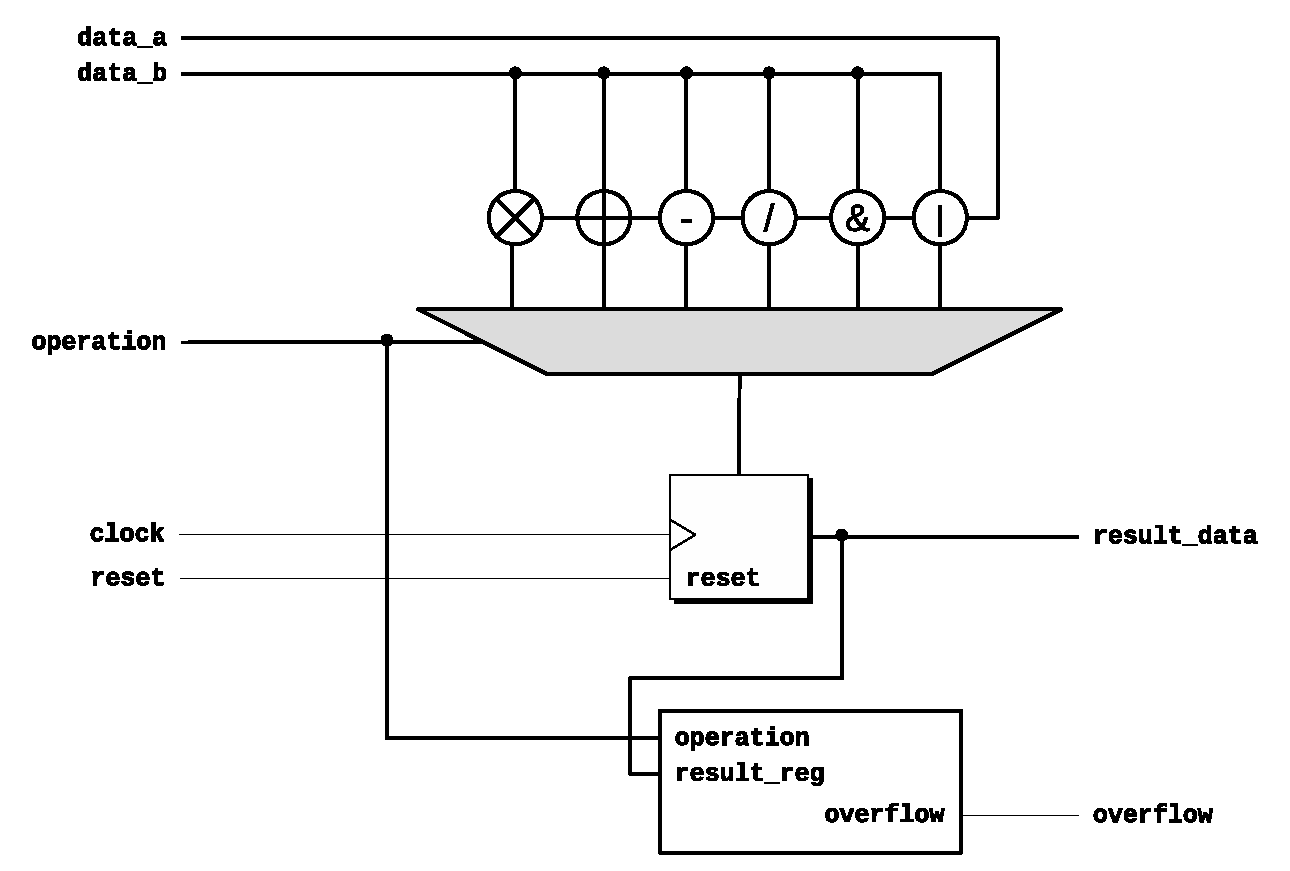
\includegraphics[width=\linewidth]{datapath/processing_datapath.eps}
      \end{figure}
    \newpage
%%%%%%%%%%%%%%%%%%%%%%%%%%%%%%%%%%%%%%%%%%%%%%%%%%%

  \section{Interface de Comunicação}

    \subsection{Diagrama de Classe}
      \begin{figure}[H]
        \centering
              \begin{tikzpicture} 
        \umlclass[type=control]{Interface\_Control}
        { % atributos
          + clock : input bit \\
          + reset : input bit \\
          + rx\_data\_ready : input bit \\
          + rx\_data : input bit[8] \\
          + data\_a : output bit[8] \\
          + data\_b : output bit[8] \\
          + operation : output bit[TBD] \\
          - state : reg bit[TBD] \\
          - data\_a\_reg : reg bit[8] \\
          - data\_b\_reg : reg bit[8] \\
          - operation\_reg : output bit[8]
        }{ % procedures
          - \underline{<<sequ>> control\_logic()} \\
          - <<sequ>> register\_assignment()
        }
      \end{tikzpicture}
      \end{figure}

    \subsection{Definições de Entrada e Saída}
      \FloatBarrier
      \begin{center}
        \begin{longtable}[pos]{| l | c | c | m{7cm} |} \hline         
          \multicolumn{1}{|c|}{\cellcolor[gray]{0.9}\textbf{Nome}} & 
          \multicolumn{1}{c|}{\cellcolor[gray]{0.9}\textbf{Tamanho}} & 
          \multicolumn{1}{c|}{\cellcolor[gray]{0.9}\textbf{Direção}} &
          \multicolumn{1}{c|}{\cellcolor[gray]{0.9}\textbf{Descrição}} \\ \hline
          \endfirsthead
          \hline
          \multicolumn{4}{|l|}%
          {{\bfseries continuação da página anterior}} \\
          \hline
          \multicolumn{1}{|c|}{\cellcolor[gray]{0.9}\textbf{Nome}} & 
          \multicolumn{1}{c|}{\cellcolor[gray]{0.9}\textbf{Tamanho}} & 
          \multicolumn{1}{c|}{\cellcolor[gray]{0.9}\textbf{Direção}} &
          \multicolumn{1}{c|}{\cellcolor[gray]{0.9}\textbf{Descrição}} \\ \hline
          \endhead

          \multicolumn{4}{|r|}{{continua na próxima página}} \\ \hline
          \endfoot

          \hline
          \endlastfoot

          clock\_in                & 1   & entrada   & Clock principal do sistema.    \\ \hline
          reset\_in                & 1   & entrada   & Sinal de reset geral do sistema.    \\ \hline
          rx\_data\_ready\_in      & 1   & entrada   & Indica que o dado foi recebido pelo controle RS232.    \\ \hline
          rx\_data\_in             & 8   & entrada   & Dado proveniente da transmissão.    \\ \hline
          data\_a\_out             & 8   & saída   & Dado do primeiro operando.    \\ \hline
          data\_b\_out             & 8   & saída   & Dado do segundo operando.    \\ \hline
          operation\_out          & TBD   & saída   & Código da operação.    \\ 
        \end{longtable}
      \end{center}    

    %\subsection{Datapath Interno}

    \subsection{Máquina de Estados}
      \begin{figure}[H]
        \centering
        \begin{tikzpicture} 
        \umlstateinitial[name=idle]
        \umlstatefinal[x=8, y=-3.2, name=final]
        \umlbasicstate[x=0, y=-4, do=counter++, name=read]{read\_data}  
        \umlbasicstate[x=4, y=-3.5, name=send]{send\_data}    

        \umltrans[arg={rx\_data\_ready\_in}]{idle}{read}
        \umltrans{read}{send}
        \umltrans{send}{final}
        \umltrans[recursive=-160|-120|3cm, recursive direction=right to bottom, arg={counter != 3}, pos=1.5]{read}{read} 
        \end{tikzpicture}    
      \end{figure}

    \begin{landscape}
      \subsection{Diagrama de Temporização}
        \begin{figure}[H]
          \centering
          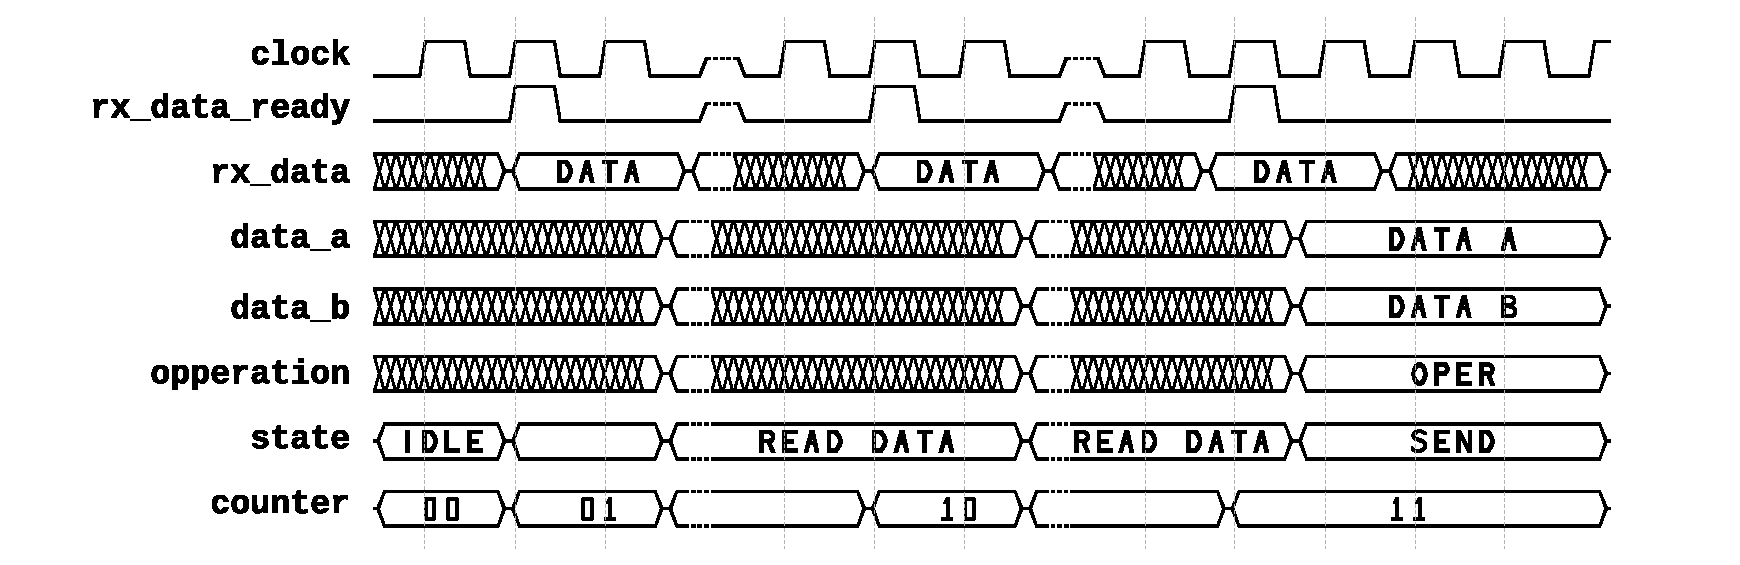
\includegraphics[width=\linewidth]{timing/comunication_timing.eps}
        \end{figure}
    \end{landscape} 

% Optional bibliography section
% To use bibliograpy, first provide the ipprocess.bib file on the root folder.
% \bibliographystyle{ieeetr}
% \bibliography{ipprocess}

\end{document}
